
\noindent\textbf{命题~\ref{prop:7-2-277} 的证明。}
证明与命题~\ref{prop:7-2-275} 类似。
事实上，可把
\[
\operatorname{Incl}_s\colon
C(L'_i,\lambda'_i)
\longrightarrow
C([0,1]_s\times L'_i,\lambda'_i)
\]
看作从恒等映射到自身的同伦。
这一同伦的构造（命题~\ref{prop:7-2-162}）
与命题~\ref{prop:7-2-160} 的证明中
$\mathfrak f^{\{\psi_{r_0,s}\}_s}$ 的构造类似。
换言之，为证明命题~\ref{prop:7-2-277}，
我们将把命题~\ref{prop:7-2-275} 的证明
应用于 $\Psi_{r,s}$ 不依赖 $r,s$、
恒等于 $\phi'$ 的情形。
但为求完整，以下仍重复给出证明细节。

考虑常值同伦 $\{\phi'\}_s$，
其中对所有 $s\in[0,1]$，
$\phi'_s=\phi'$。
它给出滤过 $A_{n,K}$ 同态
\begin{equation}
\mathfrak f^{\{\phi'\}_s}\colon
C(L'_0,\lambda'_0)
\longrightarrow
C([0,1]_s\times L'_1,
(\lambda'_0,\lambda'_1)),
\tag{7.2.345}\label{eq:7-2-345}
\end{equation}
且满足
\begin{equation}
\operatorname{Eval}_{s=s_0}\circ
\mathfrak f^{\{\phi'\}_s}
=\mathfrak f^{\phi'}.
\tag{7.2.346}\label{eq:7-2-346}
\end{equation}
注意，为定义 (7.2.345)，
可能需要向引理~\ref{lem:7-2-300}
所定义的
$C([0,1]_s\times L'_1,
(\lambda'_0,\lambda'_1))$
增添更多单形。
然而，命题~\ref{prop:7-2-277} 与
命题~\ref{prop:7-2-275} 的证明实际上可以同步进行。
这样便可在证明引理~\ref{lem:7-2-300} 的阶段，
固定 $C([0,1]_s\times L'_1,
(\lambda'_0,\lambda'_1))$ 的选取，
使 (7.2.345) 已有定义。
为简便起见，以下假定两处使用同一个
$C([0,1]_s\times L'_1,
(\lambda'_0,\lambda'_1))$。

\begin{lemma}{7.2.347}\label{lem:7-2-347}
存在滤过 $A_{n',K'}$ 代数
\[
C_1([0,1]^2\times L'_1,
(\lambda'_0,\lambda'_1)),
\]
它是 $[0,1]^2\times
C(L'_1,(\lambda'_0,\lambda'_1))$
的 $A_{n',K'}$ 类模型；
还存在滤过 $A_{n',K'}$ 同态
\[
\widetilde{\mathfrak H}_1\colon
C(L'_0,\lambda'_0)
\longrightarrow
C_1([0,1]^2\times L'_1,
(\lambda'_0,\lambda'_1)),
\]
满足
\begin{equation}
\operatorname{Eval}_{s=s_0}
\circ\widetilde{\mathfrak H}_1
=\operatorname{Incl}_r\circ\mathfrak f^{\phi'},
\tag{7.2.348}\label{eq:7-2-348}
\end{equation}
且下列图式~\ref{diag:7-2-30} 交换：

\par\medskip\noindent\begin{minipage}{\textwidth}
\centering
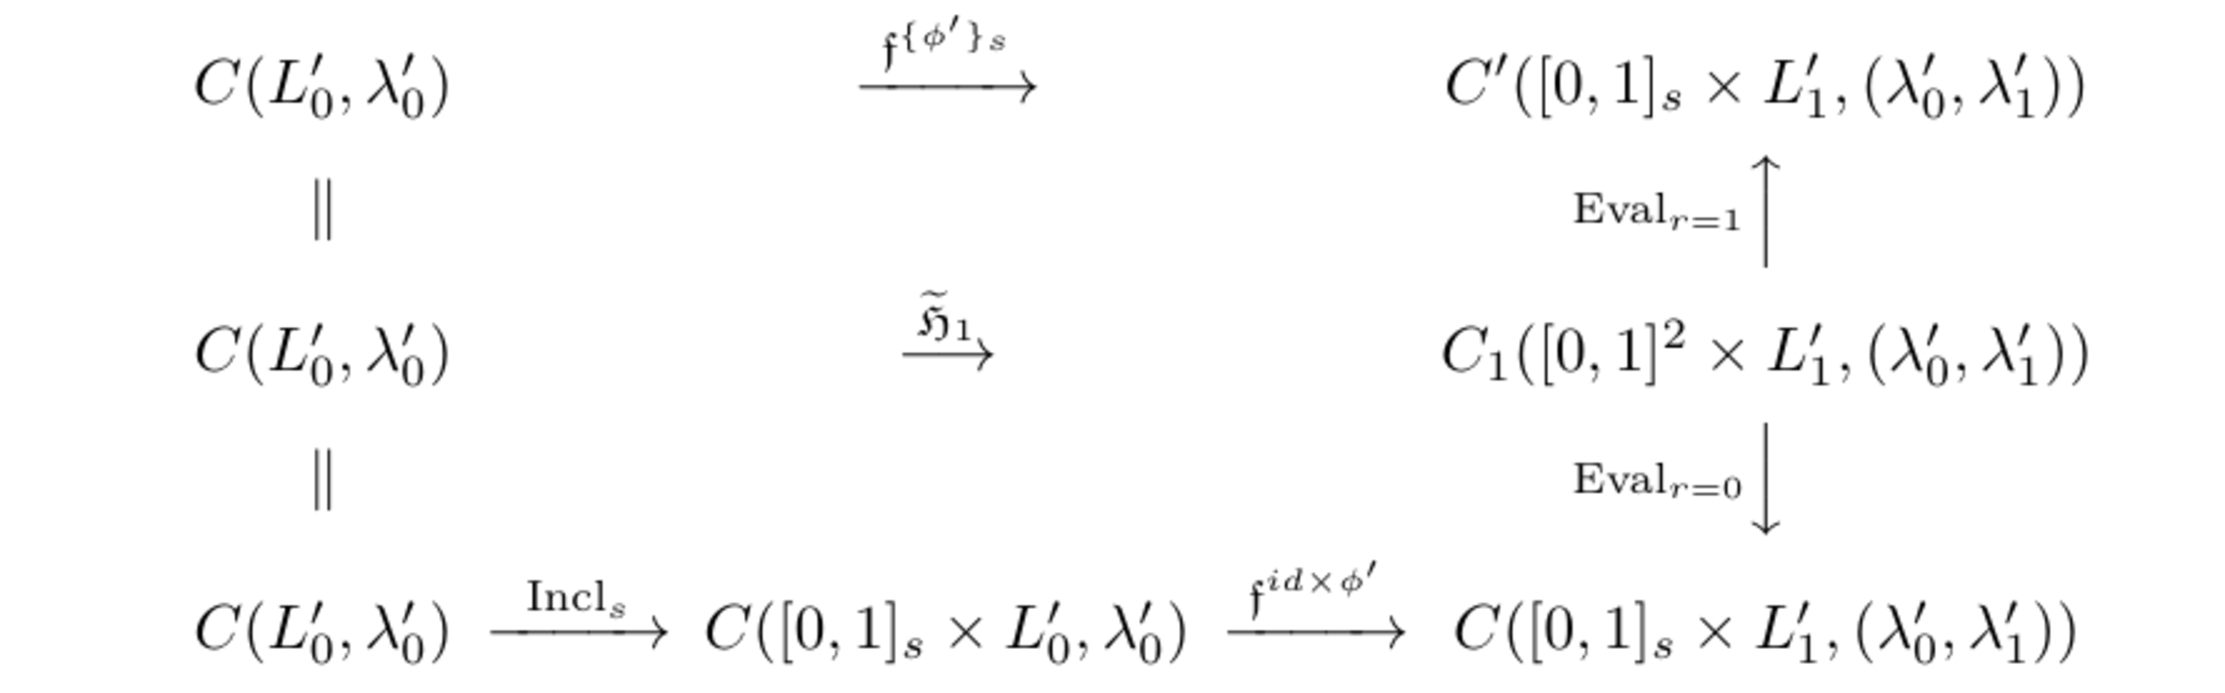
\includegraphics[width=\textwidth]{chapters/ch07-transversality/figures/phys-575-diagram-7-2-30-math-final-crop.png}
\par{\renewcommand{\thefigure}{7.2.30}\refstepcounter{figure}
\normalfont\bfseries 图式~\thefigure\label{diag:7-2-30}}
\end{minipage}\par\medskip
这里，$C([0,1]_s\times L'_1,
(\lambda'_0,\lambda'_1))$
由引理~\ref{lem:7-2-300} 构造；
$C'([0,1]_s\times L'_1,
(\lambda'_0,\lambda'_1))$
则是
$[0,1]\times C(L'_1,
(\lambda'_0,\lambda'_1))$
的模型，由适配奇异单形构成的适当可数子复形
在几何上构造而得。
\end{lemma}

\noindent\textbf{证明。}
证明与引理~\ref{lem:7-2-328} 类似。
图式~\ref{diag:7-2-30} 的底行映射
由引理~\ref{lem:7-2-300} 构造，
顶行映射由第 7.2.10 小节构造。
为构造满足 (7.2.348) 的
$\widetilde{\mathfrak H}_1$，
考虑下列交换图式：

\par\medskip\noindent\begin{minipage}{\textwidth}
\centering
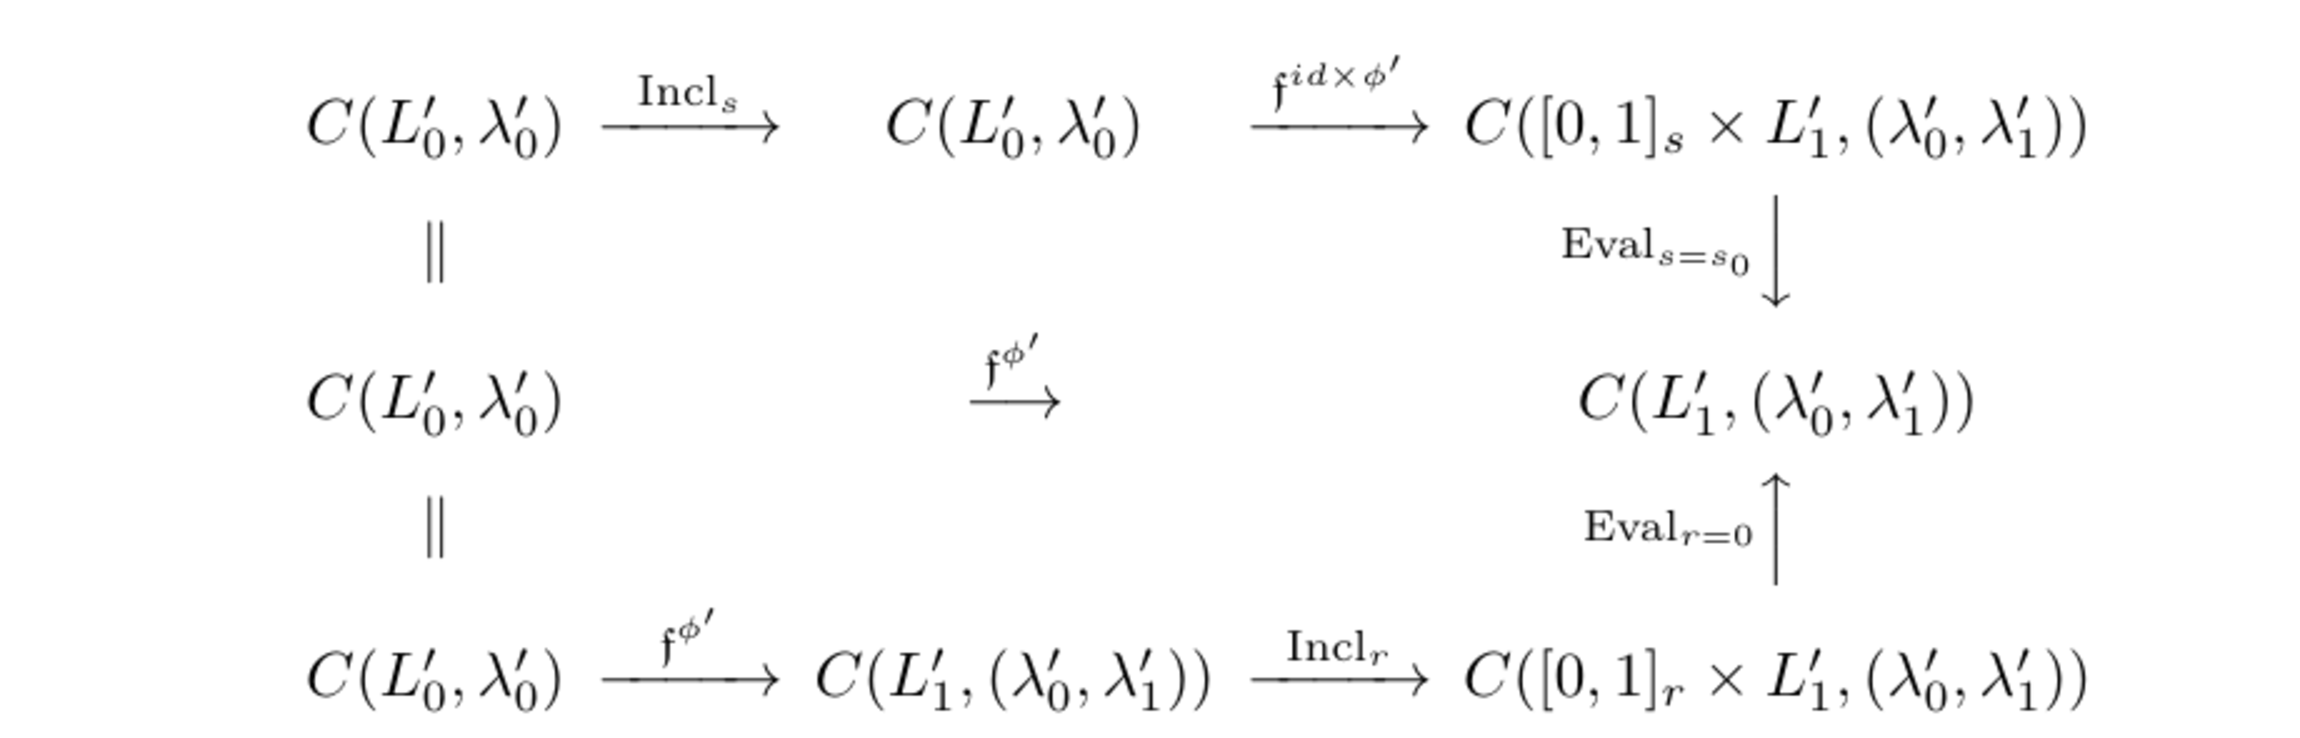
\includegraphics[width=\textwidth]{chapters/ch07-transversality/figures/phys-576-diagram-7-2-31-math-final2-crop.png}
\par{\renewcommand{\thefigure}{7.2.31}\refstepcounter{figure}
\normalfont\bfseries 图式~\thefigure\label{diag:7-2-31}}
\end{minipage}\par\medskip
图式~\ref{diag:7-2-31} 的上行中点
保留源书标注\translatornote{上行 $\operatorname{Incl}_s$
的靶写作 $C(L'_0,\lambda'_0)$；
按图式 7.2.30 底行及随后
$\mathfrak f^{\operatorname{id}\times\phi'}$
的定义域，应为
$C([0,1]_s\times L'_0,\lambda'_0)$。
此处保留原图，提示其型别不合。}。

\par\medskip\noindent\begin{minipage}{\textwidth}
\centering
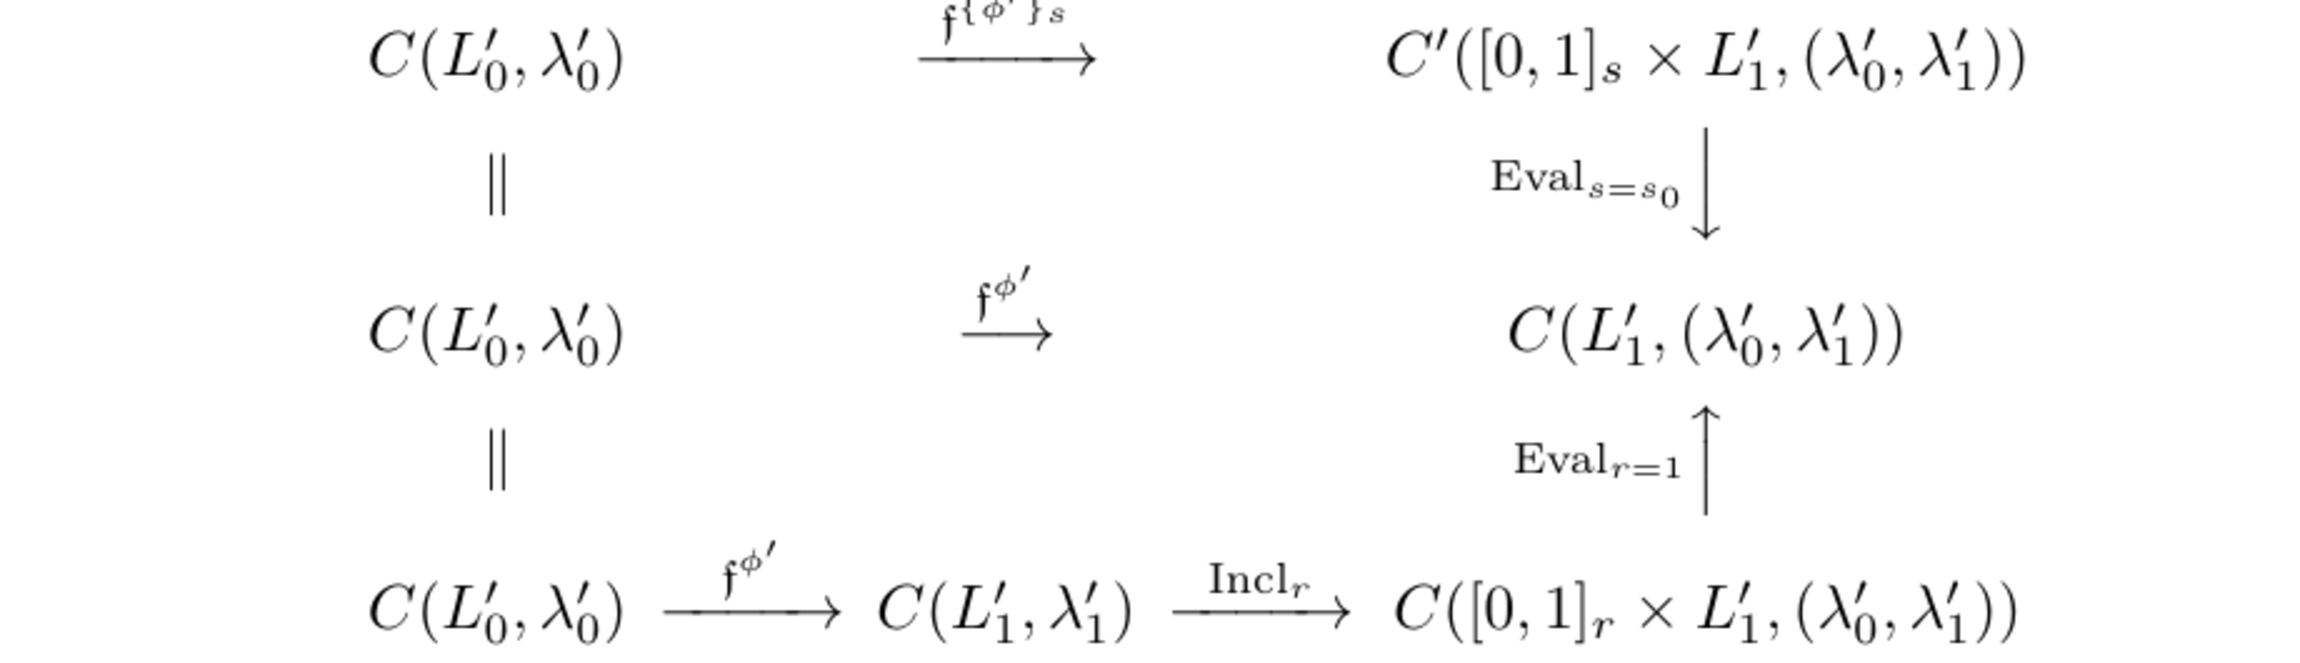
\includegraphics[width=\textwidth]{chapters/ch07-transversality/figures/phys-576-diagram-7-2-32-math-final-crop.png}
\par{\renewcommand{\thefigure}{7.2.32}\refstepcounter{figure}
\normalfont\bfseries 图式~\thefigure\label{diag:7-2-32}}
\end{minipage}\par\medskip
图式~\ref{diag:7-2-32} 的底行标注亦保留原样
\translatornote{底行的 $\mathfrak f^{\phi'}$ 指向
$C(L'_1,\lambda'_1)$，而 (7.2.346)
及图式 7.2.31 使用
$C(L'_1,(\lambda'_0,\lambda'_1))$。
此处暂不判定是箭头还是靶模型误植。}。

图式~\ref{diag:7-2-31}、\ref{diag:7-2-32}
的交换性表明，可在
$\partial[0,1]^2\times L'_1$ 上
构造 $C_1([0,1]^2\times L'_1,
(\lambda'_0,\lambda'_1))$
及 $\widetilde{\mathfrak H}_1$
（即在相应模空间上构造适当的多值截面）。
随后可按照引理~\ref{lem:7-2-285} 的证明方式，
把构造扩张至内部；
也就是说，把这些多值截面延拓到内部。

注意，此处给出的是几何证明；
并未使用纯代数的命题~\ref{prop:7-2-312}。
原因是，难以找到一个滤过 $A_{n,K}$ 代数
充当命题~\ref{prop:7-2-312} 前提中的 $C_0$。
这里转而使用扰动模空间的参数空间可缩这一事实。\qed
